\documentclass[a4paper]{article}
\usepackage{amsmath}
\usepackage{stmaryrd}
\addtolength{\hoffset}{-2.25cm}
\addtolength{\textwidth}{4.5cm}
\addtolength{\voffset}{-3.25cm}
\addtolength{\textheight}{5cm}
\setlength{\parindent}{15pt}

\usepackage[unicode=true, colorlinks=false, hidelinks]{hyperref}
\usepackage[utf8]{inputenc}
\usepackage[english, russian]{babel}
\usepackage{mathtext}
\usepackage[T2A, TS1]{fontenc}
\usepackage{microtype} % Slightly tweak font spacing for aesthetics
\usepackage{amsthm, amssymb, amsmath, amsfonts, nccmath}
\usepackage{nicefrac}
\usepackage{epstopdf}
\usepackage[export]{adjustbox}
\usepackage{float} % Improved interface for floating objects
\usepackage{graphicx, multicol} % Enhanced support for graphics
\usepackage{pdfrender,xcolor}
\usepackage{breqn}
\usepackage{mathtools}
\usepackage{titling}
\usepackage{bm}
\usepackage{centernot}
\usepackage[cal=boondoxo,calscaled=.96]{mathalpha}
\usepackage{marvosym, wasysym} % More symbols
\usepackage{rotating} % Rotation tools
\usepackage{censor} % Facilities for controlling restricted text

\usepackage{fancyhdr}
\pagestyle{fancy}
\fancyhead{}\renewcommand{\headrulewidth}{0pt}
\fancyfoot[L]{}
\fancyhead{}
\fancyfoot{}
\fancyfoot[R]{\thepage}
\begin{document}
    \begin{titlepage}
   \begin{center}
       \vspace*{3cm}
       \large{САНКТ-ПЕТЕРБУРГСКИЙ ПОЛИТЕХНИЧЕСКИЙ УНИВЕРСИТЕТ}
       \vspace{0.4 cm}

       \large\textbf{Институт прикладной математики и механики}
       \vspace{0.4 cm}

       \large{Высшая школа прикладной математики и вычислительной физики}

       \vspace{3 cm}
       \normalsize\textbf{Отчет\\ по лабораторной работе №7\\ по дисциплине\\
«Математическая статистика»}
       \vfill
       \begin{flushright}
            \normalsize{Выполнил студент:\\
            Антонов Алексей\\
            группа: 3630102/80201}
            \vskip\medskipamount
            \normalsize{Проверил:

            к.ф.-м.н., доцент\\
            Баженов Александр Николаевич
            }
       \end{flushright}

       \vspace{0.8cm}


       \normalsize{Санкт-Петербург\\2021 г.}

   \end{center}
\end{titlepage}
    \tableofcontents
    \newpage
	\listoffigures
    \newpage
    \listoftables
    \newpage

\section {Постановка задачи}
\noindent Провести дисперсионный анализ с применением крритерия Фишера по данным регистраторов для одного сигнала.
Определить области однородности сигнала, переходные области, шум/ фон.
Длину сигнала взять равной 1024.

\section{Теория}
\subsection{Критерий Фишера}
Критерий фишера относится к критериям рассеяния. Пусть заданы две выборки:
$$x^n = (x_1, x_2, ..., x_n),\ x_i \in \mathbb{R} \ \forall i = \overline{1, n}$$
$$y^m = (y_1, y_2, ..., y_m),\ y_i \in \mathbb{R} \ \forall i = \overline{1, m}$$
\\
Обозначим дисперсии выборок как $\sigma_1^2, \ \sigma_2^2$ и выборочные оценки дисперсий как $s_1^2, \ s_2^2$. \\
\\
Дополнительное предположение: выборки $x^n$ и $y^m$ являются нормальными. Критерий Фишера чувствителен к нарушению предположения о нормальности.\\
\\
Нулевая гипотеза $H_0$ - справедливость выражения $s_1^2 = s_2^2$. Статистика критерия Фишера: $F = \frac{s_1^2}{s_2^2}$ - имеет распределение Фишера с n-1 и m-1 степенями свободы. Обычно в числителе ставится большая из двух сравниваемых дисперсий. Тогда критической областью критерия является правый хвост распределения Фишера, что соотвествует альтернативной гипотезе $H_1^'$: $s_1^2 > s_2^2$. Пусть $H_1$: $s_1^2 \neq s_2^2.$\\
\\
Критерий при уровне значимости $\alpha$:
\begin{itemize}
    \item если $F < F_{\alpha/2}(n-1, m-1)$ или $F > F_{1 - \alpha/2}(n-1, m-1)$, то нулевая гипотеза $H_0$ отвергается в пользу альтернативы $H_1$;

    \item если $F > F_{1 - \alpha}(n-1, m-1)$, то нулевая гипотеза $H_0$ отвергается в пользу альтернативы $H_1^'$.
\end{itemize}
Здесь $F_{\alpha}(n-1, m-1)$ - $\alpha$ квартиль распределения Фишера с n-1 и m-1 степенями свободы.

\subsection{Внутригрупповая дисперсия}
\begin{equation}
    s_{IntaGroup}^2 = \frac{1}{k} \sum_{i=1}^k s_i^2 = \frac{1}{k} \sum_{i=1}^k \frac{\sum_{j=1}^n (x_{ij} - X_m)^2}{k-1},
\end{equation}
где $X_m$ - среднее для части выборки, $k$ - количество частей выборки, $n$ - количество элементов в рассматриваемой части выборки.\\
\\
Внутригрупповая дисперсия является дисперсией совокупности и рассматривается как среднее значение выборочных дисперсий.

\subsection{Межгрупповая дисперсия}
\begin{equation}
    s_{InterGroup}^2 = k \frac{\sum_{j=1}^k (X_{im} - X_m)^2}{k-1},
\end{equation}
где $X_im$ - среднее для под-выборок, $k$ - количество частей выборки, $X_m$ - среднее значение этих средних значений под-выборок.\\

\subsection{Определение областей однородности сигнала}
Мы будем сравнивать межгруповую и внутригруповую дисперсии по критерию Фишера. Если значение критерия Фишера велико, это будут переходные процессы, если же значение находится вблизи 1, то эти области однородны.


\section{Программная реализация}
\noindent Лабораторная работа выполнена на языке Python в среде PyCharm с использованием следующих библиотек:
 \begin{enumerate}
        \item math
        \item matplotlib
        \item numpy
 \end{enumerate}

\section{Результаты}
	\begin{figure}[H]
		\centering
		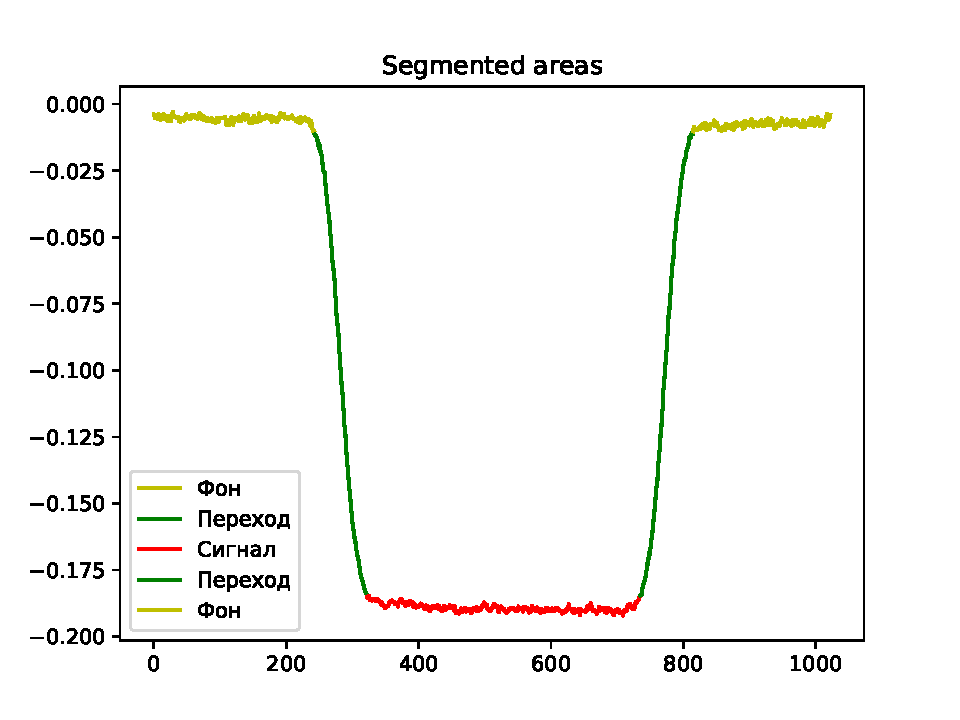
\includegraphics[width = 13cm, height = 8cm]{src/Segmented500}
		\caption{Изображение входного сигнала}
		\label{fig:signal}
	\end{figure}

		\begin{figure}[H]
		\centering
		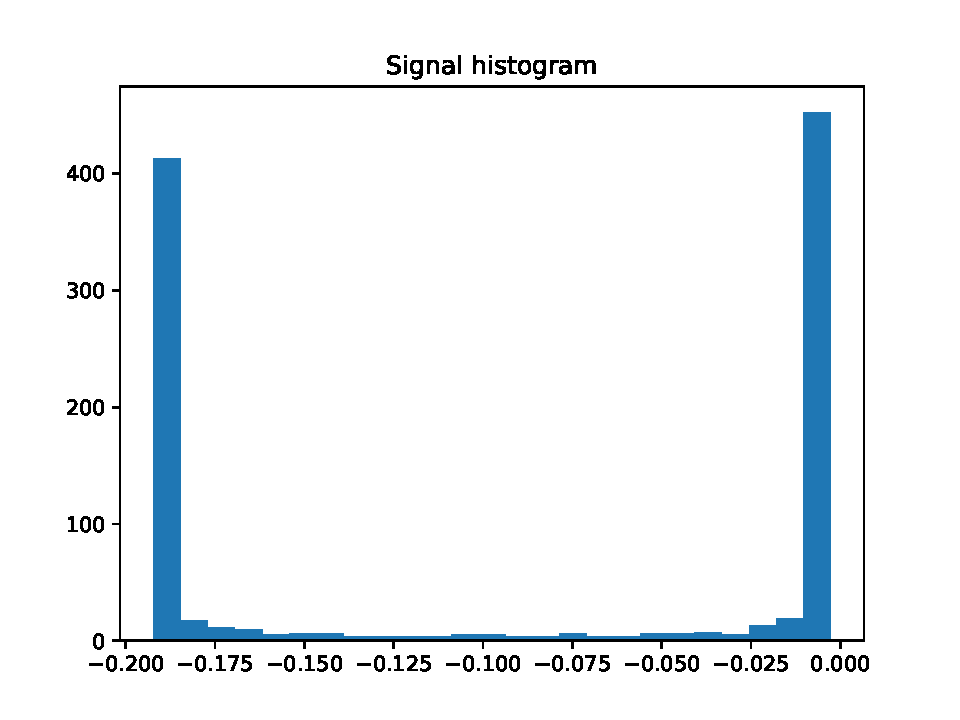
\includegraphics[width = 13cm, height = 8cm]{src/Signal500Hist}
		\caption{Гистограмма сигнала}
		\label{fig:signalHist}
	\end{figure}

	\begin{figure}[H]
		\centering
		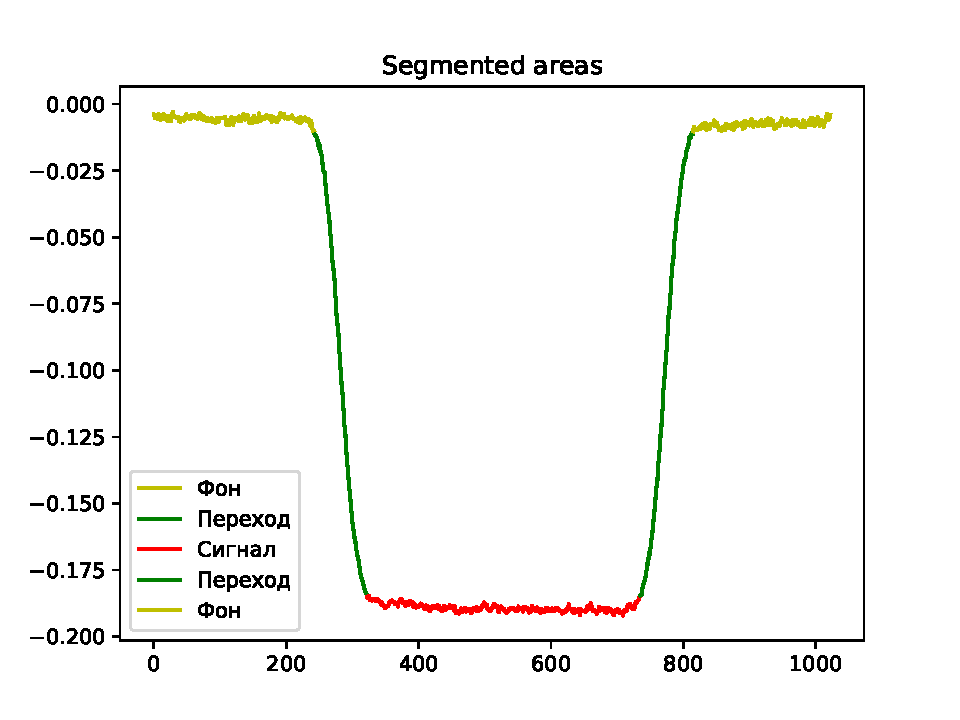
\includegraphics[width = 13cm, height = 8cm]{src/Segmented500}
		\caption{Разделение областей для данных сигнала}
		\label{fig:signalSegmented}
	\end{figure}
	\begin{table}[H]
    \centering
    \begin{tabular}{|c|c|c|c|}
    	\hline
        Промежуток&Тип&Количество разбиений&Критерий Фишера\\ \hline
1&Фон&9&1.3668\\ \hline
2&Переход&4&19.3068\\ \hline
3&Сигнал&7&1.0187\\ \hline
4&Переход&4&19.5921\\ \hline
5&Фон&4&0.1866\\ \hline

    \end{tabular}
    \caption{Характеристики выделенных областей}
    \label{tab:FisherTab}
\end{table}
\section{Обсуждение}
\subsection{Проверка гипотезы о законе распределения генеральной совокупности. Метод хи-квадрат}

\noindent Заключаем, что гипотеза $H_{0}$ о нормальном законе распределения $N(x,\hat{\mu}, \hat{\sigma})$ на уровне значимости $\alpha = 0.05$ согласуется с выборкой для нормального распределения $N(x, 0, 1)$.
\\
Также видно, что для выборок сгенерированных по равномерному закону и закону Лапласа гипотеза $H_{0}$ оказалась принята.

\section{Приложение}
    С кодом работы и отчета можно ознакомиться по ссылке:\;\url{https://github.com/sqrtyyy/MathStat/tree/master/lab_8}

\end{document}
